\documentclass[../report.tex]{subfiles}
\begin{document}
\graphicspath{{img/}{../img/}}

The storage layer is implemented with different design patterns, but the overall architecture is built around the object-mapper pattern. This means that the storage layer doesn't know anything about the object model. This is done so that if a new entity were to be added, only the object model has to been updated in order to implement the change. 

%Write about extensible data structure

The structure of the DAL (See figure \ref{DALclassdiagram}) have been implemented to support NFR-07 and NFR-08. The DAL is abstracting concrete implementation from the Business Logic Layer through a bridge pattern. This have been done so that persistence modules can be swapped, without changes in the layer above, if the persistence needs to be updated or changed to another technology. 

A relational database management module have been implemented using Entity Framework. Entity framework is a good choice as it supports easy access to the database. The performance of EF is not as well as hard coded SQL-queries, but it's much more flexible and dynamic. The EF module are using the transaction state pattern to ensure that the database is consistent. The state pattern keeps track of the entities states, and only when Save Changes is invoked, the data is actually saved to the persistent module. This ensures that if the program were to crash while working on ongoing transactions, the persistent data integrity would not be violated. To improve performance while using the EF the database uses foreign keys which the entity framework uses for making property references for easy mapping between objects.

\begin{figure}
\centering
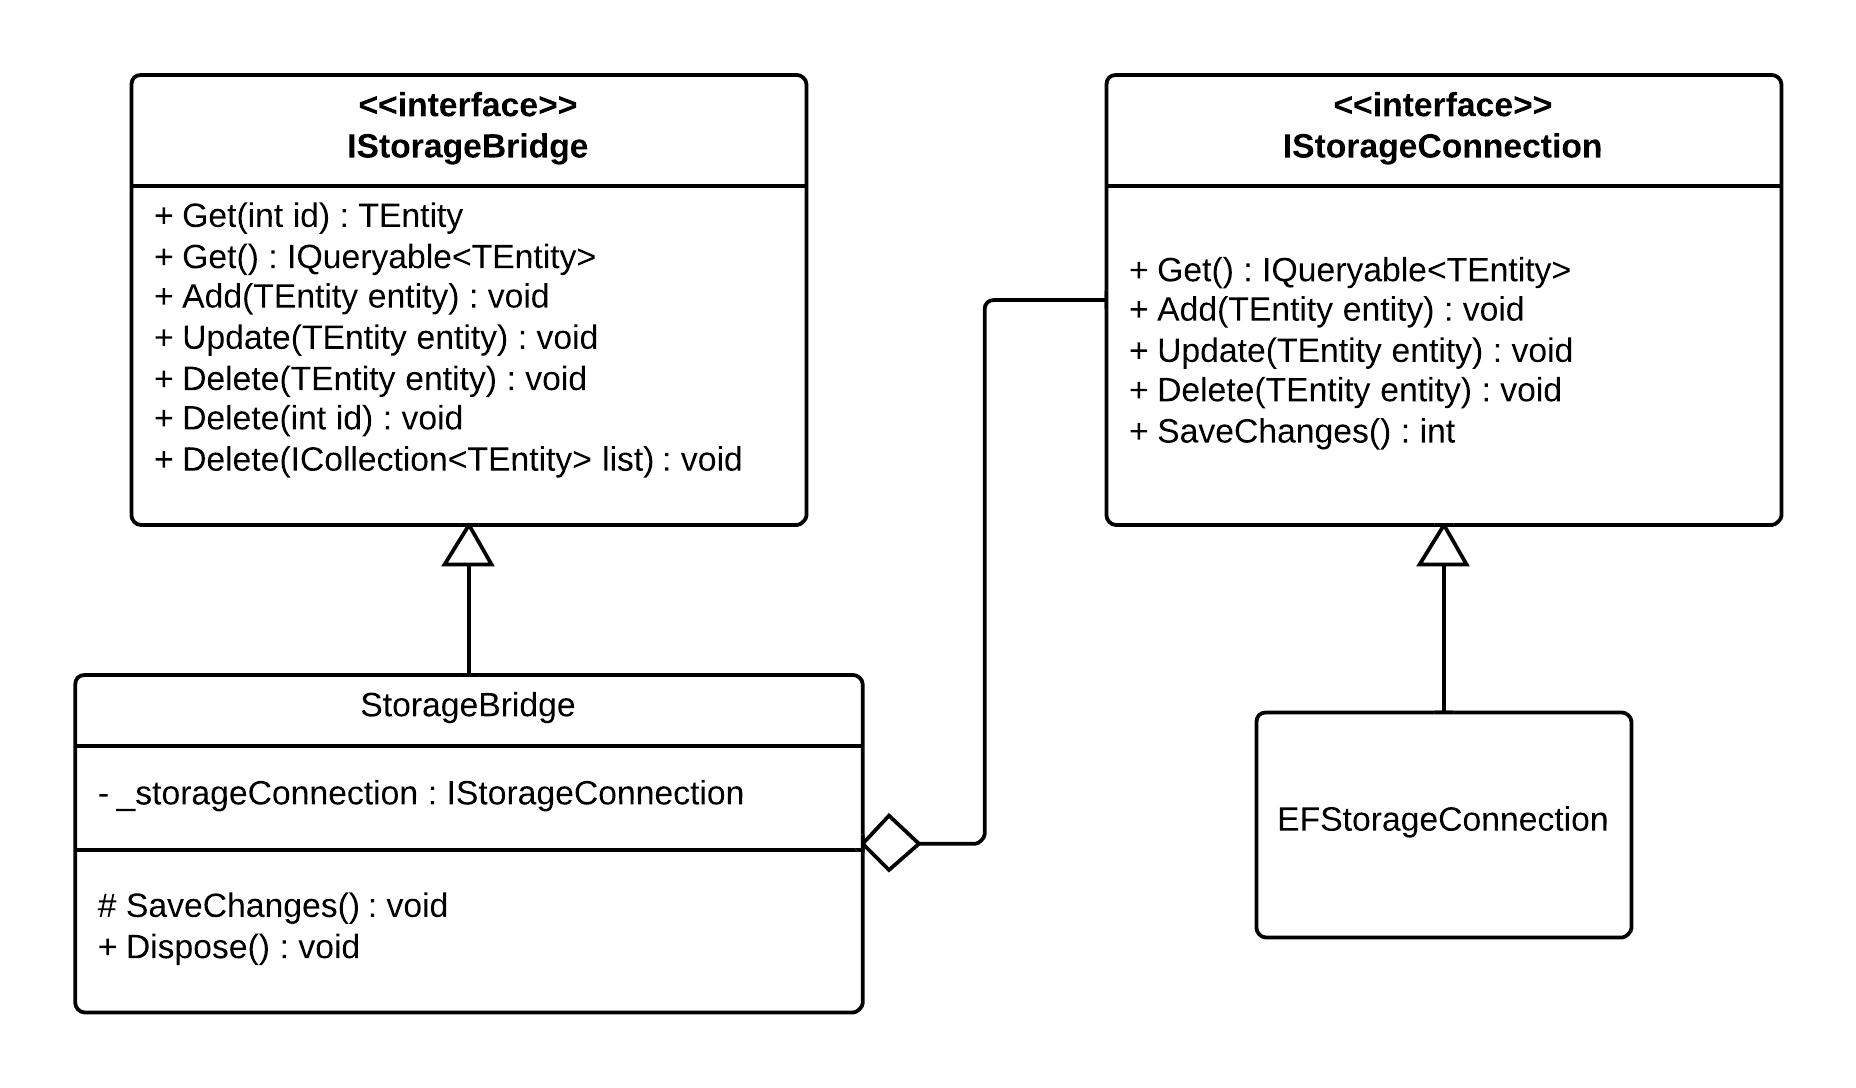
\includegraphics[width=\linewidth]{DALclassdiagram.png}
\caption{Data Access Layer architecture}
\label{fig:DALclassdiagram}
\end{figure} 

\end{document}